\documentclass[12pt,a4paper]{article}
\usepackage[latin1]{inputenc}
\usepackage[spanish]{babel}
\usepackage{amsmath}
\usepackage{amsfonts}
\usepackage{amssymb}
\usepackage{makeidx}
\usepackage{graphicx}
\usepackage[left=2cm,right=2cm,top=2cm,bottom=2cm]{geometry}
\author{MEJORADA LOPEZ IVAN}
\title{parametros de circuitos de activacion y transistores dde potencia }
\begin{document}
\maketitle

\includegraphics[width=16cm]{UPZMG_Prueba_1b.png}  
\newpage
\section{QUE ES UN PARAMETRO}
Se conoce como par''ametro al dato que se considera como imprescindible y orientativo para lograr evaluar o valorar una determinada situaci\'on. A partir de un par\'ametro, una cierta circunstancia puede comprenderse o ubicarse en perspectiva. Por dar algunos ejemplos concretos: “\Si nos basamos en los par\'ametros habituales, resultar\'a imposible comprender esta situaci\'on”, “El paciente est\'a evolucionando de acuerdo a los par\'ametros esperados\”, \“ Estamos investigando pero no hay par\'ametros que nos permitan establecer una relaci\'on con el caso anterior\”, “La actuaci\'on del equipo en el torneo local es el mejor par\'ametro para realizar un pron\'ostico sobre su participaci\'on en el campeonato mundial \”.

\section{parametros electronicos fundamentales}
Si se aproximan una barra de ebonita a otra de vidrio, se comprobar\'a que no existe ning\'un efecto entre ellas (ni atracci\'on ni repulsi\'on). Si luego se las frota y se las acerca una contra otra se notaran los efectos de atracci\'on. Se dice entonces que los cuerpos est\'an electrizados y
se puede concluir que la electrizaci\'on se produjo por frotamiento. A \'este tipo de electricidad se la denomina est\'atica. Todos estamos familiarizados con los efectos de la electricidad est\'atica
incluso algunas personas son m\'as susceptibles que otras a su influencia. Para explicar como se origina la electricidad est\'atica, hemos de considerar que la materia est\'a compuesta de \'atomos, y los \'atomos de part\'iculas cargadas, de modo de que queda conformada por un n\'ucleo compuesto por protones con carga positiva y de neutrones carentes de carga el\'ectrica, rodeado de una nube de electrones que tienen carga negativa. Normalmente, la materia es neutra, tiene el mismo n\'umero de cargas positivas (protones) y negativas (electrones).\\ 
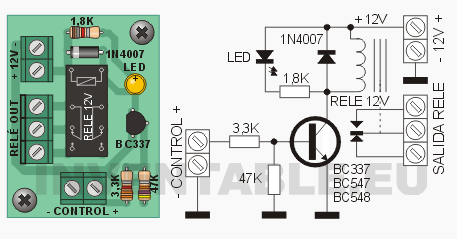
\includegraphics[width=13cm]{conexion-rele-transistor.png} 
\newpage
\section{funcionamiento}
El funcionamiento y utilizaci\'on de los transistores de potencia es id\'ntico al de los transistores normales, teniendo como caracter\'isticas especiales las altas tensiones e intensidades que tienen que soportar y, por tanto, las altas potencias a disipar.

Existen tres tipos de transistores de potencia:\\

*bipolar.\\
*unipolar o FET (Transistor de Efecto de Campo).\\
*IGBT.\\

\section{IGBT}
El IGBT ofrece a los usuarios las ventajas de entrada MOS, m\'as la capacidad de carga en corriente de los transistores bipolares\\

Cuando el transistor est\'a en saturaci\'on o en corte las p\'erdidas son despreciables. Pero si tenemos en cuenta los efectos de retardo de conmutaci\'on, al cambiar de un estado a otro se produce un pico de potencia disipada, ya que en esos instantes el producto IC x VCE va a tener un valor apreciable, por lo que la potencia media de p\'erdidas en el transistor va a ser mayor. Estas p\'erdidas aumentan con la frecuencia de trabajo, debido a que al aumentar \'esta, tambi\'en lo hace el n\'emero de veces que se produce el paso de un estado a otro.\\

\end{document}